\section{Related work}\label{related-work}

\subsection{Information analysis workflow}

Pirolli and Card's Think Loop Model \cite{Pirolli2005} is a widely used model of information analysis. The model describes the process of information foraging and sensemaking in which raw evidence is successively modeled, filtered, and synthesized into a best hypothesis. The model is a bottom-up process of structure building, but also includes a local feedback loop at each stage. Thus, analysts can reconsider propositions in the evidence file, asking how they are related, or a given hypothesis, asking what schemata it rests upon.

Empirical studies of information analysis suggest that the iterative looping can
have a wider scope than is obvious in the Pirolli and Card's model
\cite{Pirolli2005}. For example, Chin et al. \cite{Chin2009} observed five
professional intelligence analysts working both individually and as a team. They
found that analysts often need to review the original documents even at advanced
stages of analysis. The scope of these reconsiderations is not consistent with
the local feedback architecture of the Think Loop Model. It seems more
consistent with a parallel or multi-phased model \cite{Wheaton2011} in which
structure building occurs at a variety of levels in parallel. Similar findings
were reported by other empirical studies
\cite{Isenberg2008b,Kang2011,Herrmann2013a}. A report \cite{Badalamente2005}
from a workshop of professional intelligence analysts listed ``dynamic data
processing and visualization'' as one of top requirements in computational
support for intelligence analysis, emphasizing the need for an integrated
environment for data modeling and analysis.

However, tools supporting information analysis are often designed targeted at a single phase of activity, and thus not supporting the whole workflow. For example, research efforts have been made to understand information collection and modeling \cite{Shah2014i, Jansen2010c}, but little support is provided to extend these models to analysis. Techniques such as Information Extraction and Weight (IEW) helps structures data evidence but offers no structure to turn the evidence to hypothesis development. Similarly, tools supporting the activity of data analysis assume data has been modeled. Analytic tools such as interactive visualization emphasize present data in insightful means but provides no utility to data re-modeling \cite{Ware2012}.

Similar calls were made in other data intensive task domains as well. For
example, in interactive machine learning, researchers \cite{Chen2016,
Amershi2015} call for an all-in-one environment in which machine learning
practitioners can tune model parameters and evaluate model performance through
visualization in one place. In the area of visual analytics, Ware
\cite{Ware2012} warned of the \emph{``asymmetry in data rates''} [p.382],
pointing out that visual analytic tools emphasized data flowing from systems to
users far more than from users to systems. Functionalities are mostly designed
to adjust data representation rather than modeling, which are in fact equally
important. Our work aligns with these efforts, and contribute to the design and
evaluation of an integrated workspace in supporting information analysis tasks.

\subsection{Collaboration and awareness in information analysis}

Collaboration is critical in information analysis. The intelligence community has called for collaboration, and indeed closer collaboration, as opposed to merely coordinating draft products by the end \cite{Vision2015}. Empirical studies \cite{Chin2009,Kang2011} reported that analysts' practice was fundamentally collaborative. Effective collaboration helps analysts pool different knowledge and expertise and reduces the effect of confirmation bias \cite{Heuer1999}.

Significant efforts have been made to understand and support collaboration in the CSCW community, and many of them address, as it is in our study, tasks with large and complex data, such as collaborative modeling \cite{Kolfschoten2008, Prilla2013}, collaborative information seeking \cite{Golovchinsky2009a, Kelly2014a}, and collaborative visualization \cite{Isenberg2011,Heer2008e}. While these works provide insight in supporting teamwork with complex artifacts, less is known in terms of how technology-mediated collaboration occurs in a complete analytic process, and what awareness is needed for analytic specific purposes.

The state-of-the-art computational tools supporting intelligence analysis either
do not support collaboration, or they do not integrate serious analytic
support. On one hand, most analytic tools (e.g.~Analyst's Notebook and PARC ACH)
are designed for single user only, with only a few exceptions (e.g.~Te@mACH
\cite{Globalytica2017}). On the other hand, as Treverton \cite{Treverton2016}
reviewed state-of-the-art collaboration tools in the intelligence community, those
tools only support coordination for general situations, without specific analytic functionalities. For example, Intellipedia
\cite{Intelink2017} is a wiki platform for sharing of intelligence reports and
documents, yet it does not integrate functions for data modeling and analysis at all.

A key enabler for effective collaboration is \emph{activity awareness}, defined as
team's awareness of its own sustained collaborative activity
\cite{Carroll2003,Carroll2006}. Derived from Activity Theory \cite{Leontev1974},
activity awareness encompasses information covering all aspects of collaboration, such as partner presence, mediating artifacts, group actions, social interactions, shared information, and group values and norms. Activity awareness has been utilized as a design concept in guiding and evaluating collaboration features.

% place system figure here simply for paper layout
\begin{figure*}
\centering
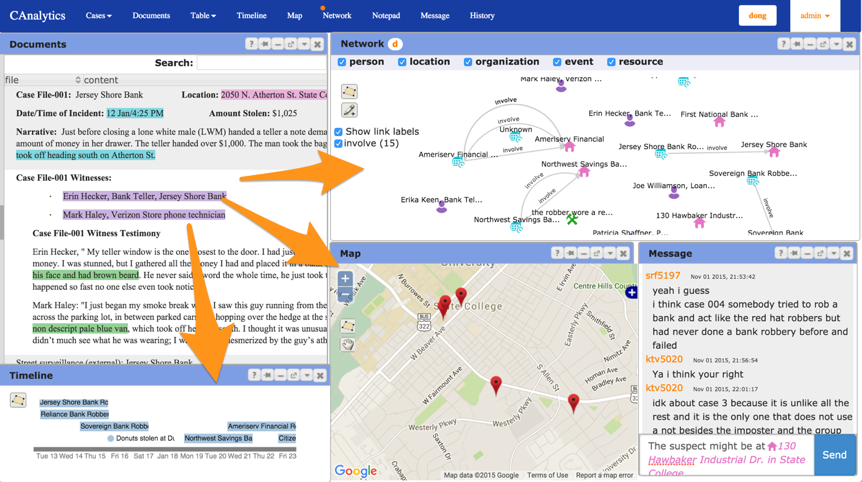
\includegraphics[width=2\columnwidth]{./img/interface.png}
\caption{CAnalytics user interface. Each window is closable, movable, and resizable. Shown here are \emph{document} view (top left), timeline (bottom left), network (top right), map (bottom middle), and message (bottom right). Other windows include table, notepad, and history view. }\label{fig:canalytics}
\end{figure*}

Many lab studies have been reported to investigate specific awareness features
to support collaboration in information analysis. For example, Convertino et
al. \cite{Convertino2011} examined the use of public and private views for role
based collaboration. Goyal and Fussell \cite{Goyal2016} studied the effect of
hypotheses sharing on sensemaking. Mahyar and Tory \cite{Mahyar2013b} designed a
visualization to connect collaborators' common findings and evaluated its
support for team performance. Hajizadeh et al. \cite{Hajizadeh2013} explored how
sharing teammate's interactions affects awareness. These studies provide
evidence to validate hypotheses of specific design features. However, due to
time constraint (mostly within one hour), these studies had to employ a
simplified task with reduced content and complexity. Artifacts created by
participants were thus relatively simple and superficial (e.g.~with a single
artifact or few items in an artifact). More complex task would have pushed
participants to create more sophisticated artifacts (e.g.~multiple views or
cluttered display that requires filtering) and to try balancing between team
coordination and individual reasoning, which would have provided more insights
into team-based analytic process. Our study aims to examine tool usage in a
classroom context, which allows for higher task complexity and longer teamwork
time in a more realistic environment.
